%-----------------------------------------------------------------------
% Beginning of chap2.tex
%-----------------------------------------------------------------------
%
%  AMS-LaTeX sample file for a chapter of a monograph, to be used with
%  an AMS monograph document class.  This is a data file input by
%  chapter.tex.
%
%  Use this file as a model for a chapter; DO NOT START BY removing its
%  contents and filling in your own text.
% 
%%%%%%%%%%%%%%%%%%%%%%%%%%%%%%%%%%%%%%%%%%%%%%%%%%%%%%%%%%%%%%%%%%%%%%%%


\chapter*{Lecture 5}
\addcontentsline{toc}{chapter}{Lecture 5}
\addtocounter{chapter}{5}
\addtocounter{section}{0}
%\numberwithin{section}{chapter}
\numberwithin{equation}{chapter}
\numberwithin{theorem}{chapter}

% \epigraph{}{--- \textup{}}

In Lecture 4 we found out that gradient descent works, and has linear convergence. In this lecture we introduce Newton's method, an algorithm that takes advantage of the second derivative and has quadratic convergence under certain circumstances. Throughout this lecture, $\norm{\cdot}$ will refer to the $2$-norm $\norm{\cdot}_2$.

\section{Newton's Method}
Let $f\in C^2(\R^n)$ and let's look again at the unconstrained problem
\begin{equation*}
 \minimize f(\vct{x}).
\end{equation*}
Newton's method starts with a guess $\vct{x}_0$ and then proceeds to compute a sequence of points $\{\vct{x}_k\}_{k\geq 0}$ in $\R^n$ by the rule
\begin{equation}\label{eq:newton}
 \vct{x}_{k+1} = \vct{x}_k - \nabla^2 f(\vct{x}_k)^{-1}\nabla f(\vct{x}_k), \quad k\geq 0.
\end{equation}
The algorithm stops when $\norm{\vct{x}_{k+1}-\vct{x}_k}<\e$ for some predefined tolerance $\e>0$.
In the context of the general scheme $\vct{x}_{k+1}=\vct{x}_k+\alpha_k\vct{p}_k$, the step length is $\alpha_k=1$, and the search direction is the inverse of the Hessian multiplied with the negative gradient. 

Recall that the inner product $\ip{\vct{p}}{\nabla f(\vct{x})}$ is the directional
derivative of $f$,
and that a {\em descent direction} is a direction in which the rate of change (slope) is negative. The following gives a criterion for the search direction in Newton's method to be a descent direction.

\begin{lemma}
Let $\mtx{B}\in \R^{n\times n}$ be a positive definite symmetric matrix and $f\in C^1(\mtx{R}^n)$.
Then $\vct{p}=-\mtx{B}^{-1}\nabla f(\vct{x})$ is a descent direction of $f$ at $\vct{x}$.
\end{lemma}

\begin{proof}
 If $\mtx{B}\in \R^{n\times n}$ is symmetric and positive definite, then $\mtx{B}^{-1}$ is also positive definite, since for all $\vct{v}\in \R^n$, 
 \begin{equation*}
  \vct{v}^{\trans}\vct{B}^{-1}\vct{v}= (\mtx{B}\vct{B}^{-1}\vct{v})^{\trans}\vct{B}^{-1}\vct{v}
  = 
  (\mtx{B}^{-1}\vct{v})^{\trans}\mtx{B}^{\trans} (\mtx{B}^{-1}\vct{v}) = (\mtx{B}^{-1}\vct{v})^{\trans}\mtx{B} (\mtx{B}^{-1}\vct{v})>0.
 \end{equation*}
(This can also be seen by noting that the eigenvalues of $\mtx{B}^{-1}$ are the inverses of the eigenvalues of $\mtx{B}$.)
 For $\vct{p}=-\mtx{B}^{-1}\nabla f(\vct{x})$ we then get
 \begin{equation*}
  \ip{\vct{p}}{\nabla f(\vct{x})} = -\ip{\vct{B}^{-1}\nabla f(\vct{x})}{\nabla f(\vct{x})} =-\nabla f(\vct{x})^{\trans}\mtx{B}^{-1}\nabla f(\vct{x})<0,
 \end{equation*}
which shows that $\vct{p}$ is a descent direction. 
\end{proof}

To better understand Newton's method, we first look at the one dimensional case. 

\begin{example}
 Let $f\in C^2(\R)$. In this case Newton's method is described as
 \begin{equation}\label{eq:newton1d}
  x_{k+1} = x_k-\frac{f'(x_k)}{f''(x_k)}, \quad k\geq 0.
 \end{equation}
Newton's method looks for a local minimizer in the form of a point $x^*$ such that $f'(x^*)=0$ and $f''(x^*)>0$. Setting $g(x):=f'(x)$, we are looking for a {\em root} $x^*$,
\begin{equation*}
 g(x^*)=0.
\end{equation*}
One approach to find such a root is to approximate the function $g(x)$ at a point $x_k$ by its tangent line,
\begin{equation*}
 g(x) \approx g(x_k)+g'(x_k)(x-x_k),
\end{equation*}
and then identify the next iterate $x_{k+1}$ as the root of this linear approximation:
\begin{equation*}
 g(x_k)+g'(x_k)(x_{k+1}-x_k)=0 \Longleftrightarrow x_{k+1} = x_k-\frac{g(x_k)}{g'(x_k)} 
\end{equation*}

\begin{figure}[h!]
\centering
 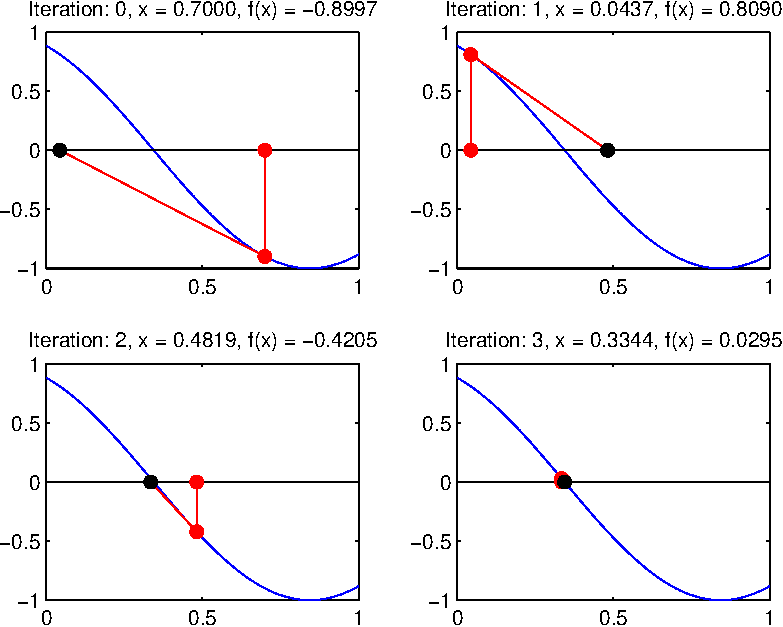
\includegraphics[width=0.6\textwidth]{images/newton-crop.pdf}
\caption{Newton's method}\label{fig:newton}
\end{figure}

Geometrically this corresponds to taking the tangent to $g$ at $x_k$ and setting $x_{k+1}$ to be the intersection of this tangent line with the $x$-axis, as shown in Figure~\ref{fig:newton}.
Replacing $g(x)=f'(x)$ gives precisely Newton's method~\eqref{eq:newton1d}.
\end{example}

Another way to understand Newton's method is to view it in contrast with gradient descent. While gradient descent corresponds to working with a {\em linear approximation}
\begin{equation*}
 f(\vct{x}_{k+1}) \approx f(\vct{x}_k)+\ip{\nabla f(\vct{x}_k)}{\vct{x}_{k+1}-\vct{x}_k},
\end{equation*}
Newton's method is based on the {\em quadratic approximation},
\begin{equation*}
 f(\vct{x}_{k+1}) \approx f(\vct{x}_k)+\ip{\nabla f(\vct{x}_k)}{\vct{x}_{k+1}-\vct{x}_k}+\frac{1}{2}\ip{\nabla^2 f(\vct{x}_k)(\vct{x}_{k+1}-\vct{x}_k)}{\vct{x}_{k+1}-\vct{x}_k}.
\end{equation*}

\begin{example}
 Consider the function $f$ on $\R^2$, 
 \begin{equation*}
  f(\vct{x}) = \frac{1}{2}(x_1^2+10x_2^2).
 \end{equation*}
Starting with $\vct{x}_0=(10,1)^{\trans}$, gradient descent takes $84$ iterations to reach accuracy $10^{-6}$, while Newton's method, unsurpringly, takes only one. 
\begin{figure}[h!]
 \centering
 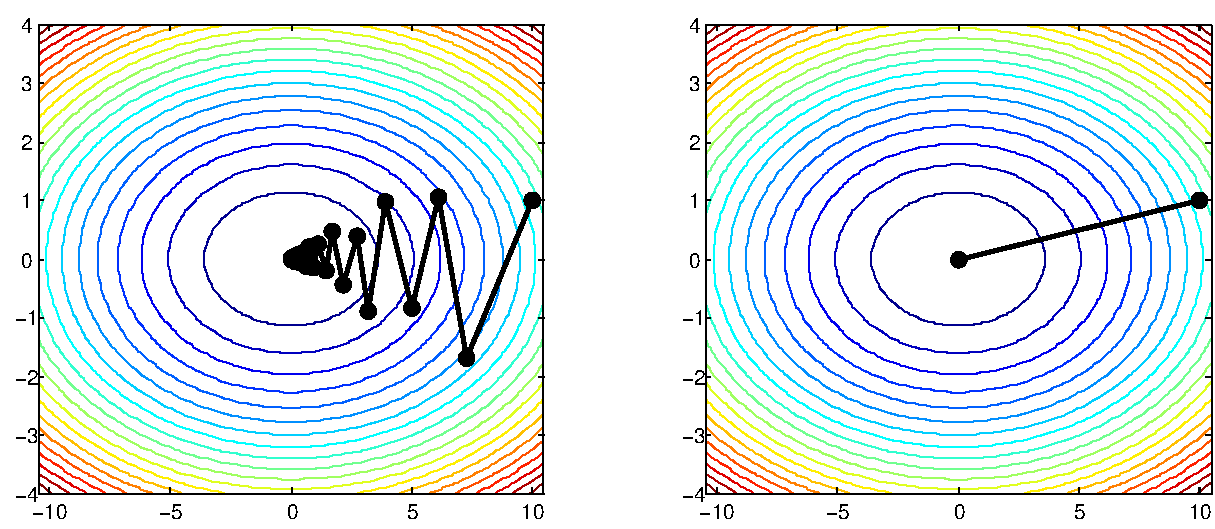
\includegraphics[width=0.7\textwidth]{images/quadnewton_cropped.pdf}
 \caption{Gradient descent vs. Newton's method on a quadratic function.}
\end{figure}
\end{example}


In practice, when implementing Newton's method one does not explicitly compute the inverse of the Hessian. The reason is that one does not need the inverse itself, but only the product $\nabla^2f(\vct{x}_k)^{-1}\nabla f(\vct{x}_k)$, which is the solution of a system of equations $\nabla^2 f(\vct{x}_k)\vct{y} = \nabla f(\vct{x}_k)$ that can be solved much more efficiently. One therefore replaces the update step~\eqref{eq:newton} with the following two steps:
\begin{align*}
 \text{ Find } \vct{y} \text{ such that   }\quad  &\nabla^2f(\vct{x}_k)\vct{y}=-\nabla f(\vct{x}_k),\\
                &\vct{x}_{k+1} = \vct{x}_k+\vct{y}.
\end{align*}

There is a lot that can go wrong with Newton's method. In particular, the matrix $\nabla^2f(\vct{x})$ has to be non-singular, or invertible, at every step. If, however, we start at a point $\vct{x}_0$ that is not too far from a local minimizer $\vct{x}^*$ with $\nabla f(\vct{x}^*)=\zerovct$ and $\nabla^2f(\vct{x}^*)$ positive definite, then we are on the safe side.

\begin{lemma}\label{le:continuity}
 Let $\vct{x}^*\in \R^n$ be such that $\nabla^2f(\vct{x}^*)$ is positive definite. Then there exists an open neighbourhood $U$ of $\vct{x}^*$ such that for all $\vct{x}\in U$, $\nabla^2 f(\vct{x})$ is positive definite.
\end{lemma}

For the main result of this lecture, namely the quadratic convergence of Newton's method, we make the additional assumption that the Hessian $\nabla^2f(\vct{x})$ is Lipschitz continuous as a function of $\vct{x}$.

\begin{definition}
 A function $f\colon \R^n\to \R^m$ is Lipschitz continuous on a domain $\Omega\subseteq \R^n$ with respect to a pair of norms on $\R^n$ and $\R^m$ if there is a constant $L>0$ such that for all $\vct{x},\vct{y}\in \Omega$,
 \begin{equation*}
  \norm{f(\vct{x})-f(\vct{y})}\leq L\norm{\vct{x}-\vct{y}}.
 \end{equation*}
 The constant $L$ is called the {\em Lipschitz constant} of the map.
\end{definition}

In particular, the Hessian of a function $f\in C^2(\R^n)$, considered as a map from $\R^n$ to $\R^{n\times n}$, is Lipschitz continuous with respect to a norm on $\R^n$ and the corresponding operator norm on $\R^{n\times n}$, 
if for any $\vct{x},\vct{y}$ we have
\begin{equation*}
 \norm{\nabla^2f(\vct{x})-\nabla^2f(\vct{y})}\leq L \norm{\vct{x}-\vct{y}}.
\end{equation*}

\begin{theorem}
 Let $f\in C^2(\R^n)$ and $\vct{x}^*\in \R^n$ a local minimizer with $\nabla f(\vct{x}^*)=\zerovct$ and $\nabla^2f(\vct{x}^*)>0$. Then for $\vct{x}_0$ sufficiently close to $\vct{x}^*$, Newton's method has quadratic convergence.
\end{theorem}

\begin{proof}(Optional)
Assume that $\nabla^2f(\vct{x}_k)$ is positive definite.
 Consider the difference
 \begin{align}\label{eq:deriv1}
 \begin{split}
  \norm{\vct{x}_{k+1}-\vct{x}^*} & = \norm{\vct{x}_{k}-\vct{x}^*-\nabla^2f(\vct{x}_k)^{-1}\nabla f(\vct{x}_k)}\\
  &\stackrel{(1)}{=} \norm{\vct{x}_{k}-\vct{x}^*-\nabla^2f(\vct{x}_k)^{-1}(\nabla f(\vct{x}_k)-\nabla f(\vct{x}^*))}\\
  &=  \norm{\nabla^2f(\vct{x}_k)^{-1}(\nabla^2f(\vct{x}_k)(\vct{x}_{k}-\vct{x}^*)-(\nabla f(\vct{x}_k)-\nabla f(\vct{x}^*))}
  \end{split}
  \end{align}
where (1) follows from $\nabla f(\vct{x}^*)=\zerovct$.
The Fundamental Theorem of Calculus tells us
\begin{align*}
 \nabla f(\vct{x}^*)-\nabla f(\vct{x}_k) &= \int_{0}^1 \frac{\diff{}}{\diff{t}} \nabla f(\vct{x}_k+t(\vct{x}^*-\vct{x}_k)) \ \diff{t}\\
 &= \int_{0}^1 \nabla^2 f(\vct{x}_k+t(\vct{x}^*-\vct{x}_k))(\vct{x}^*-\vct{x}_k) \ \diff{t}.
\end{align*}
Continuing from~\eqref{eq:deriv1}, by inserting this identity,
\begin{align*}
 \norm{\vct{x}_{k+1}-\vct{x}^*} &= \left\|\nabla^2f(\vct{x}_k)^{-1}\int_{0}^1\left[\nabla^2f(\vct{x}_k)- \nabla^2 f(\vct{x}_k+t(\vct{x}^*-\vct{x}_k))\right](\vct{x}_k-\vct{x}^*) \ \diff{t}\right\|\\
 &\leq \norm{\nabla^2f(\vct{x}_k)^{-1}}\cdot \\
 & \quad \int_{0}^1\norm{\nabla^2f(\vct{x}_k)- \nabla^2 f(\vct{x}_k+t(\vct{x}^*-\vct{x}_k))}\ \diff{t} \cdot \norm{(\vct{x}_k-\vct{x}^*)}.
\end{align*}
Applying the Lipschitz bound to the term inside the integral gives
\begin{equation*}
 \norm{\nabla^2f(\vct{x}_k)- \nabla^2 f(\vct{x}_k+t(\vct{x}^*-\vct{x}_k))} \leq L t\norm{\vct{x}_k-\vct{x}^*}.
\end{equation*}
Integrating this out, we end up with the bound
\begin{equation*}
 \norm{\vct{x}_{k+1}-\vct{x}^*} \leq \frac{L}{2}\norm{\nabla^2f(\vct{x}_k)^{-1}}\cdot \norm{\vct{x}_k-\vct{x}^*}^2.
\end{equation*}
The only remaining issue is that the ``constant'' on the right-hand side is not a constant. However, the Lipschitz continuity implies that $\nabla^2f(\vct{x}_k)$ converges to $\nabla^2f(\vct{x}^*)$ if $\vct{x}_k$ converges to $\vct{x}^*$. Since the inversion of a matrix is a continuous operation, also $\nabla^2f(\vct{x}_k)^{-1}$ converges to $\nabla^2 f(\vct{x}^*)^{-1}$. In particular, if $\vct{x}_k$ is sufficiently close to $\vct{x}^*$, we have $\norm{\nabla^2f(\vct{x}_k)^{-1}}\leq 2\norm{\nabla^2f(\vct{x}^*)}$. Setting $M:=L\norm{\nabla^2f(\vct{x}^*)^{-1}}/2$, we end up with the bound
\begin{equation*}
 \norm{\vct{x}_{k+1}-\vct{x}^*} \leq M\cdot \norm{\vct{x}_k-\vct{x}^*}^2.
\end{equation*}
By Lemma~\ref{le:continuity} there exists an open neighbourhood around $\vct{x}^*$ in which $\nabla^2f(\vct{x})$ is positive definite, and within this neighbourhood there is an $\vct{x}_0$ such that $\norm{\vct{x}_0-\vct{x}^*}^2<1/M$, which ensures that all following iterates remain in $U$. This shows quadratic convergence. 
\end{proof}

Note that the conditions for quadratic convergence in an open neighbourhood $U$ of $\vct{x}^*$ are precisely that $f$ is convex on $U$.

\section{Quasinewton methods}
One drawback of Newton's method is that it requires the computation of the Hessian matrix, which can be expensive.
Quasinewton methods use an approximation of the Hessian, $\mtx{B}_k\approx \nabla f(\vct{x}_k)$, at each step of the algorithm. These are construction in a way that $\mtx{B}_{k+1}$ can easily be computed from $\mtx{B}_k$. A popular method, that is used often in practical applications because of its efficiency, is the \textbf{Broyden-Fletcher-Shanno-Goldfarb} (\textbf{BFGS}) method. The BFGS method may be described as follows.

\begin{itemize}
\item Start with $\vct{x}_0$, $\mtx{B}_0$.
\item For $k\geq 0$, compute
\begin{align*}
  \vct{p}_k &= \mtx{B}^{-1}_k \nabla f(\vct{x}_k)\\
  \vct{x}_{k+1} &= \vct{x}_k + \alpha_k \vct{p}_k \text{ for a suitable step length } \alpha_k\\
  \vct{s}_k &= \alpha_k \vct{p}_k\\
  \vct{y}_k &= \nabla f(\vct{x}_{k+1})-\nabla f(\vct{x}_k)\\
  \mtx{B}_{k+1} &= \mtx{B}_k+\frac{\vct{y}_k\vct{y}_k^{\trans}}{\vct{y}_k^{\trans}\vct{s}_k}-\frac{\mtx{B}_k\vct{s}_k\vct{s}_k^{\trans}\mtx{B}_k}{\vct{s}_k^{\trans}\mtx{B}_k\vct{s}_k}. 
\end{align*}
\item Stop if $\norm{\nabla f(\vct{x}_k)}<\e$ for some tolerance $\e$, or if $\norm{\vct{x}_{k+1}-\vct{x}_k}<\e$. 
\end{itemize}


%\begin{example}
%In this example we compare the behaviour of gradient descent, Newton's method, and the BFGS method for minimizing the Rosenbrock function
%\begin{equation*}
%  f(x_1,x_2) = 
%\end{equation*}
% 
%\end{example}

% \hrulefill
% 
% \section*{Appendix}
% 
% We give a complete proof of Lemma~\ref{le:continuity}, the reason being that this is a nontrivial fact that is used a lot, but for which it is not easy to find a self-contained proof in the literature. We begin with an elementary observation, whose proof is an exercise (what can go wrong if the number of functions in the Lemma is not finite?)
% 
% \begin{lemma}
%  If $f_1,\dots,f_m$ are continuous functions on $\R^d$, then
% \begin{equation*}
%  g(\vct{x}) = \min_{1\leq i\leq m} f_i(\vct{x})
% \end{equation*}
% is also continuous. 
% \end{lemma}
% 
% % \begin{proof}
% %  Fix $\vct{x}$. If there exists an index $i$ such that $f_i(\vct{x})<f_j(\vct{x})$ for $j\neq i$, then $g=f_i$ in a neighbourhood of $\vct{x}$ and is therefore continuous at $\vct{x}$. If there are $k$ indices such that $f_{i_1}(\vct{x})=\cdots =f_{i_k}(\vct{x})<f_j(\vct{x})$, $j\not\in \{i_1,\dots,i_k\}$, then there is a neighbourhood $U$ of $\vct{x}$ in which $f_{i}(\vct{y})<f_j(\vct{y})$ for $i\in \{i_1,\dots,i_k\}$ and $j\not\in \{i_1,\dots,i_k\}$. 
% %  For all $\delta>0$ there exist $\e_1,\dots,\e_k>0$ such that $\norm{\vct{x}-\vct{y}}<\e_i$ implies $|f_i(\vct{x})-f(\vct{y})|<\delta$. 
% %  Let $\e<\min_i \e_i$ be such that the $\e$-ball around $\vct{x}$ is contained in $U$,
% %  and let $\vct{y}$ be such that $\norm{\vct{x}-\vct{y}}<\e$.
% %  Then there exists an index $i\in \{i_1,\dots,i_k\}$ such that $g(\vct{y}) = f_i(\vct{y})$, and
% %  \begin{equation*}
% %   |g(\vct{x})-g(\vct{y})| = |f_i(\vct{x})-f_i(\vct{y})|<\delta.
% %  \end{equation*}
% % This was to be shown.
% % \end{proof}
% 
% 
% \begin{proof}[Proof of Lemma~\ref{le:continuity}]
% For $\vct{v}\in S^{d-1}$ define the function $\sigma_{\vct{v}}(\vct{x}) = \ip{\vct{v}}{\nabla^2 f(\vct{x})\vct{v}}$ and set $\sigma(\vct{x}):=\min_{\vct{v}\in S^{d-1}}\sigma_{\vct{v}}(\vct{x})$.
% By assumption, $\sigma_{\vct{v}}(\vct{x}^*)>0$. Also by assumption, the second derivatives of $f$ are continuous functions, and as the composition of continuous functions is continuous, so is $\sigma_{\vct{v}}(\vct{x})$ at $\vct{x}^*$. 
% 
% Set $\delta = \sigma_{\vct{v}}(\vct{x}^*)/2$. By the definition of continuity, there exists an $\e(\vct{v})>0$ such that for all $\vct{x}$ with $\norm{\vct{x}-\vct{x}^*}_2<\e(\vct{v})$, $|f(\vct{x})-f(\vct{x}^*)|<\delta$ holds, which in turn implies $f(\vct{x})>0$ if $\norm{\vct{x}-\vct{x}^*}_2<\e(\vct{v})$. 
% \end{proof}
% %-----------------------------------------------------------------------
% % End of chap1.tex
% %-----------------------------------------------------------------------
